\documentclass[tikz,border=8pt]{standalone}
\usetikzlibrary{arrows.meta,calc}
\begin{document}
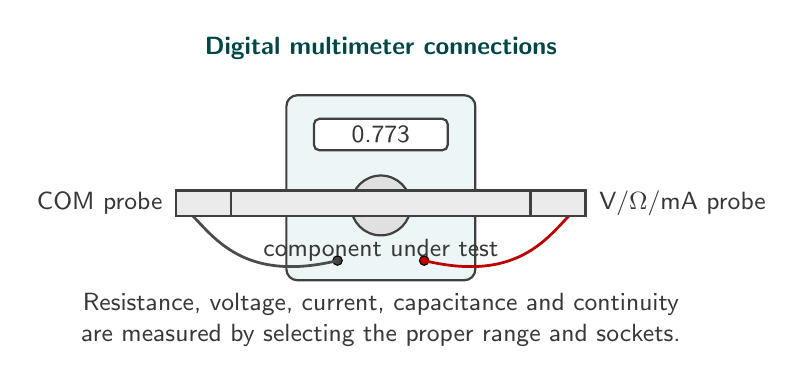
\begin{tikzpicture}[
  line/.style={draw=black!75,line width=0.8pt},
  lead/.style={draw=black!70,line width=1pt},
  label/.style={font=\sffamily\small,text=black!78},
  title/.style={font=\sffamily\bfseries\small,text=teal!55!black},
]
\node[title] at (0,3.15) {Digital multimeter connections};
\draw[line,fill=teal!7,rounded corners=4pt] (-1.2,0.2) rectangle (1.2,2.55);
\draw[line,fill=white,rounded corners=2pt] (-0.85,1.85) rectangle (0.85,2.25);
\node[label] at (0,2.05) {0.773};
\draw[line,fill=black!12] (0,1.15) circle (0.38);
\node[label] at (0,1.15) {$\Omega/V/A$};
\draw[fill=black!75] (-0.55,0.45) circle (0.06);
\draw[fill=red!75!black] (0.55,0.45) circle (0.06);
\draw[lead] (-0.55,0.45) .. controls (-2.0,0.1) and (-2.25,1.05) .. (-2.6,1.18);
\draw[lead,red!75!black] (0.55,0.45) .. controls (2.0,0.1) and (2.25,1.05) .. (2.6,1.18);
\draw[line,fill=black!8] (-2.6,1.02) rectangle (2.6,1.34);
\draw[line] (-1.9,1.02) -- (-1.9,1.34);
\draw[line] (1.9,1.02) -- (1.9,1.34);
\node[label,below] at (0,0.85) {component under test};
\node[label,left] at (-2.65,1.18) {COM probe};
\node[label,right] at (2.65,1.18) {V/$\Omega$/mA probe};
\node[label,align=center,text width=8.6cm] at (0,-0.3)
  {Resistance, voltage, current, capacitance and continuity are measured by selecting the proper range and sockets.};
\end{tikzpicture}
\end{document}
